%%%%%%%%%%%%%%%%%%%%%%%%%%%%%%%%%%
% Ch2 : Macro and micro balances %
%%%%%%%%%%%%%%%%%%%%%%%%%%%%%%%%%%$

\chapter{Macroscopic and microscopic balances}
\section{Conservation principles}
	The basic conservation principles in fluid mechanics are the conservation of \textbf{mass, energy and momentum.} These conservations are the basis of \textbf{continuity, Bernouilli and Navier-Stokes equations} and can be written in \textbf{integral} (finite volume of a mouving fluid) or \textbf{local} (balances in differential form) form. 
	
	\subsection{Macroscopic mass balance and continuity equation}
		\begin{wrapfigure}[4]{l}{4.5cm}
		\vspace{-5mm}
		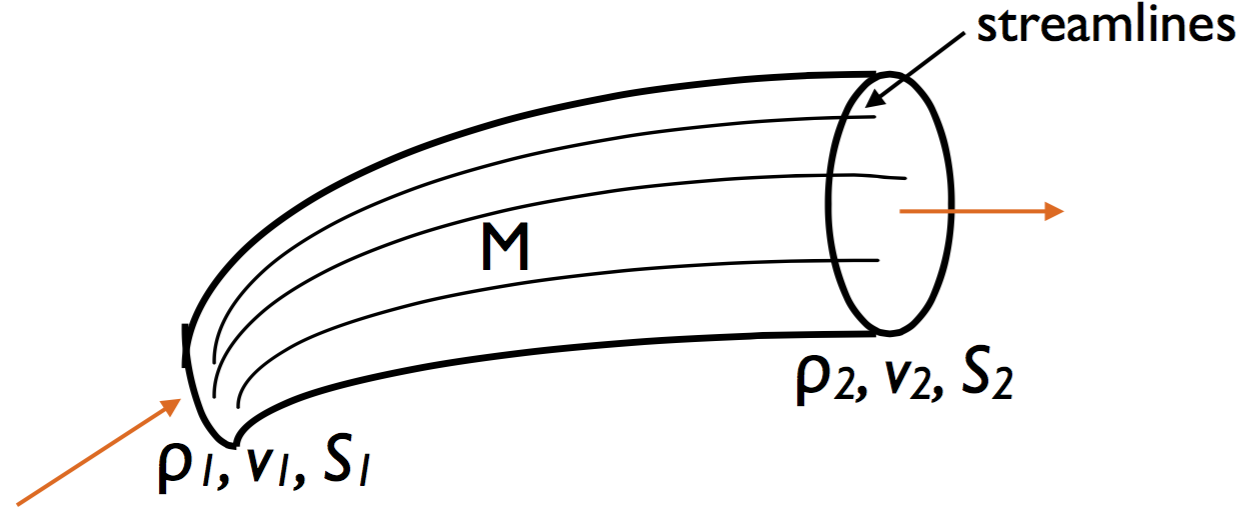
\includegraphics[scale=0.20]{ch2/1}
		\end{wrapfigure}
		In a steady\footnote{Continu, constant.} flow, the mass balance simply states that the mass entering is equal to the one leaving a volume. But we have to consider the variation of mass for transient\footnote{Transitoire.} problems. We define for that the  \textbf{mass flow rate} (débit) that gives the mass per time and is easy to measure. 
		\begin{equation}
			\dot{m} = \rho v S \qquad \qquad [\dot{m}] = \frac{[M]}{[T]}
		\end{equation}
		
		\subsubsection{General balance}
		Let's write what we explained, the mass variation is given by the mass entering at $S_1$ minus mass leaving at $S_2$		
		\begin{equation}
			\frac{dM}{dt} = \left(\rho \int _{S} v dS\right)_1 - \left(\rho \int _{S} v dS\right)_2
		\end{equation}
		To simplify, we introduce the \textbf{average velocity} $\bar{v} = \frac{1}{S}\int _S vdS$	giving the final expression
		\begin{equation}
			\frac{dM}{dt} = \left(\rho \bar{v} S\right)_1 - \left(\rho \bar{v} S\right)_2
		\end{equation}

		\subsubsection{Steady balance}
			When the fluid is steady, the velocity and the syrface are constant in both 2 sections conducting to a constant mass
			\begin{equation}
				\dot{m} = \rho \bar{v}S = c
			\end{equation}

		\subsubsection{Streamlines}
			\begin{wrapfigure}[10]{r}{4.5cm}
			\vspace{-5mm}
			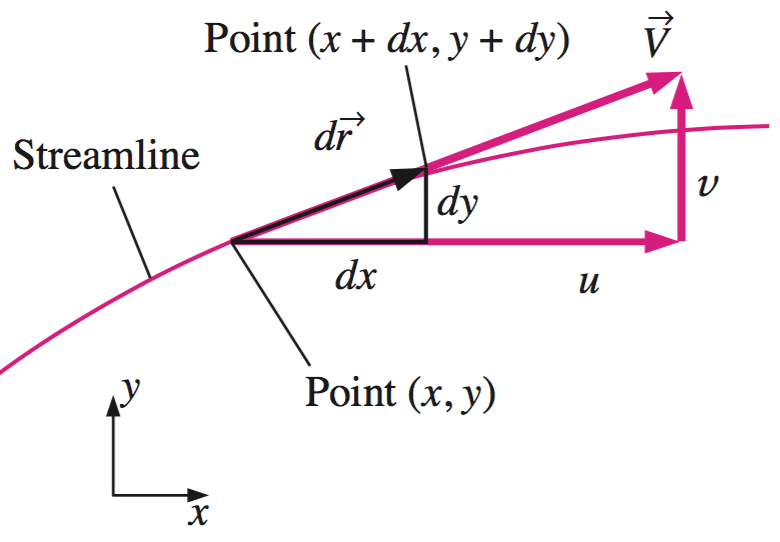
\includegraphics[scale=0.35]{ch2/2}
			\end{wrapfigure}
			Let's first define what's a streamline. It's a curve that is everywhere tangent to the instantaneous local velocity vector and so an indicator of the fluid direction. 
			Mathematically, if our velocity vector is 
			\begin{equation}
				\vec{V} = u\vec{i}+v\vec{j}+w\vec{k}
			\end{equation}
			we can take an infinetisimal arc length along a streamline 
			\begin{equation}
				d\vec{r} = dx\vec{i}+dy\vec{j}+dz\vec{k}
			\end{equation}
			Due to the 2 similar triangles, we have the relations \autoref{eq:2.4} that gives the 2D equation of a streamline.
			\begin{equation}
				\frac{dr}{V} = \frac{dx}{u} = \frac{dy}{v} = \frac{dz}{w} \qquad
				 \Rightarrow \qquad
				 \left(\frac{dy}{dx}\right)_{\mbox{along a streamline}} = \frac{v}{u}
				\label{eq:2.4}
			\end{equation}
			
	\subsection{Macroscopic momentum balance}
		Unlike the mass, momentum can be created and destroyed due to applied forces. The difference between the moementum entering in the control volume at $S_1$ and leaving at $S_2$ is equal to the sum of the forces applied to the fluid element. \\
		The momentum flow through a section per unit time is given by 
		\begin{equation}
			\dot{Q} = \dot{m}v = \rho \bar{v}^2 S
		\end{equation}
			
			